\documentclass[10pt]{article}
\usepackage[margin=0.62in]{geometry}
\usepackage[T1]{fontenc}
\usepackage{xurl,hyperref,graphicx}
\hypersetup{hidelinks}
\setlength{\parindent}{0pt}\setlength{\parskip}{4pt}
\begin{document}\small
\textbf{EXP-ECDLP-3c166b: original native execution observation}\\
RUN-ECDLP-4a3ca0 \quad GOAL-ECDLP-001 \quad H-ECDLP-85fe43

Observations only. No scientific verdict, hypothesis transition or attack claim is made. One deterministic original worksheet ran; its driver and checker both exited 0. Native schema validation then recorded \texttt{invalid\_output}.

\begin{minipage}[t]{0.59\linewidth}\vspace{0pt}
\textbf{Recorded execution.} Requested 1; driver completed 1; checker completed 1; supervisor-valid 0; invalid-output 1; no recorded timeout.\\
\textbf{Commit:} \path{ef69e0a04ce0fbbc9ecd00d5e25fa5493aece47b}\\
\textbf{Platform:} linux. Python: 3.12.14 (main, Aug 25 2026, 14:00:49) [Clang 22.1.3 ]. Dirty-tree state and CPU/GPU model at launch were unrecorded.\\
\textbf{Memory limit:} 256MiB; actual peak RSS and CPU seconds unrecorded.\\
\textbf{Derived wall interval:} 0.138067seconds from native receipt finish minus start; includes driver/checker/schema processing. n=1; uncertainty unreported; no timing comparison.\\
\textbf{Metrics copied from original manifest:} \{"beyond\_matrix": false, "matrix\_holds": true, "planted\_ok": true\}
\end{minipage}\hfill\begin{minipage}[t]{0.37\linewidth}\vspace{0pt}\centering
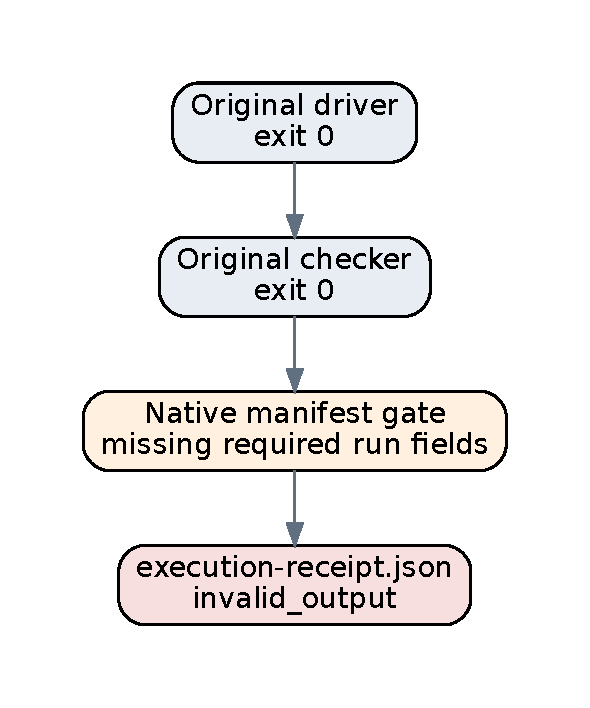
\includegraphics[height=2.7in,width=\linewidth,keepaspectratio]{diagram.pdf}\\
\footnotesize RUN-ECDLP-4a3ca0, n=1. One wall interval and no two comparable scientific measurements; therefore a process diagram is used.
\end{minipage}

\textbf{Native refusal.} manifest.yaml fails the run schema (tools/validate\_ledger.py): bad run id None; run missing required field 'id'; run missing required field 'status'; run missing required field 'code'; run missing required field 'environment'; run missing required field 'inputs'; run missing required field 'timing'; run missing required field 'result'; run.code.commit missing (not reproducible); run.code.command missing (not reproducible); run.result.certificate.kind must be one of discrete\_log|decomposition|none

\textbf{Exact inputs.} \{"curves": [\{"equation": "y\textasciicircum{}2 = x\textasciicircum{}3 - x + 1", "expected\_high": 16, "expected\_low": 20, "expected\_projective": 37, "name": "E1"\}, \{"equation": "y\textasciicircum{}2 = x\textasciicircum{}3 + x", "expected\_high": 9, "expected\_low": 10, "expected\_projective": 20, "name": "E2"\}], "expected\_gap": 3, "low\_end": 14, "named\_future\_run\_slot": "RUN-ECDLP-4a3ca0", "prime": 29\}

\textbf{Exact argv (repository root working directory).}\\
{\footnotesize \path{python3}\\
\path{experiments/EXP-ECDLP-3c166b/implementation/run.py}\\
\path{--trial-plan}\\
\path{experiments/EXP-ECDLP-3c166b/trial-plan.json}\\
\path{--run-dir}\\
\path{/workspace/crypto-autoresearcher/experiments/EXP-ECDLP-3c166b/runs/RUN-ECDLP-4a3ca0}}

\textbf{Controls, seeds and missing evidence.} The unchanged source checker ran the frozen controls and exited 0; all controls, original seed labels and raw-artifact hashes are in \path{facts.json} and the original specification. No new sample or re-scoring was introduced. The obsolete manifest lacks a certificate declaration; raw output claims no attack. Schema or checker acceptance alone does not establish execution proof or independent scientific correctness.

\textbf{Sources and next action.} Native receipt: \path{experiments/EXP-ECDLP-3c166b/runs/RUN-ECDLP-4a3ca0/execution-receipt.json}. Exact provenance, input/control lists and artifact digests: \path{facts.json}. Fresh separately approved reproduction: EXP-ECDLP-11c54d / RUN-ECDLP-d9188a; original predictions stay in-sample calibration. Original failed artifacts stay immutable. No canonical scientific graph is changed.
\end{document}
